% $Id%

\enlargethispage{1cm}
\section{CrypTool-Men"us}
\hypertarget{appendix-menutree}{}\label{s:appendix-menutree}
Dieser Anhang enth"alt den kompletten Men"u-Baum von CrypTool. Bitte beachten
Sie, dass nicht immer alle Men"ueintr"age gleichzeitig verf"ugbar sind, weil 
der Men"ubaum dynamisch aufgebaut wird. Welche Men"ueintr"age gerade
angezeigt werden, bestimmt das aktive Dokumentenfenster. So ist z.~B.
die Brute-Force Analyse f"ur DES nur verf"ugbar, wenn das aktive Fenster in
Hexadezimal-Darstellung ge"offnet ist, w"ahrend der Men"ueintrag 
"`Zufallsdaten erzeugen\dots"' immer verf"ugbar ist. In den Abbildungen
\ref{menu-detail-1} und \ref{menu-detail-2} ist dieser Zusammenhang 
hinter den Men"ueintr"agen in eckigen Klammern dargestellt,
z.~B. bedeutet "`Suchen\dots[ATH]"', dass die Funktion "`Suchen\dots"' nur f"ur
ASC-, Text- und Hexadezimal-Fenster verf"ugbar ist.
\begin{center}
\begin{tabular}{rl}
\bf Codebuchstabe & \bf Dokumententyp \\
M & (kein Dokument ge"offnet)\\
A & ASC\\
T & Text\\
H & Hexadezimal\\
P & Plot\\
\end{tabular}
\end{center}

\nobreak

\begin{figure}[!hb]
\begin{center}
\includegraphics[scale=1.1, clip, viewport=10 360 400 600]{figures/cryptool-menu-detail-de}
\caption{Detaillierte Ansicht des CrypTool-Men"u-Baums -- Teil 1}
\label{menu-detail-1}
\end{center}
\end{figure}

\begin{figure}[b]
\begin{center}
\includegraphics[scale=1.1, clip, viewport=400 190 784 598]{figures/cryptool-menu-detail-de}
\caption{Detaillierte Ansicht des CrypTool-Men"u-Baums -- Teil 2}
\label{menu-detail-2}
\end{center}
\end{figure}

\begin{figure}[hb]
\begin{center}
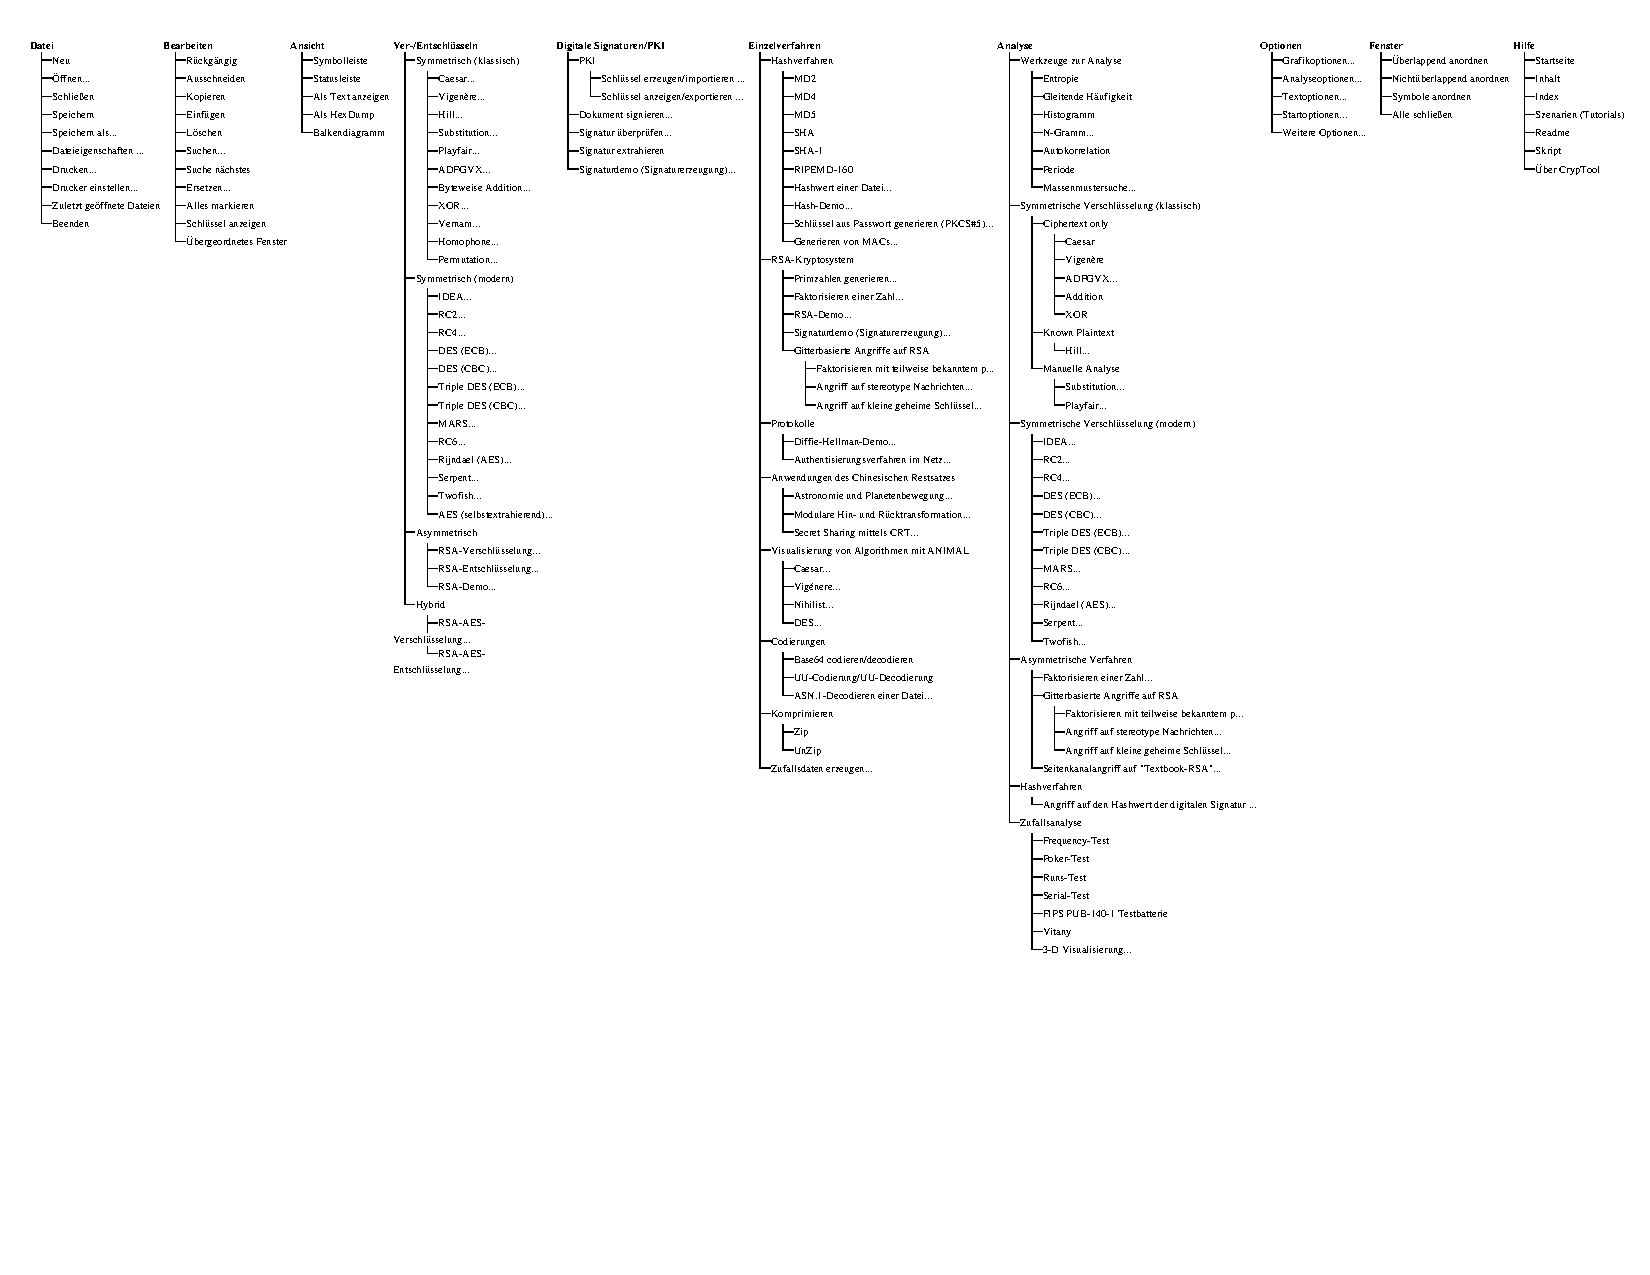
\includegraphics[scale=0.75, angle=270, viewport=14 107 779 590]{figures/cryptool-menu-de}
\vspace{-18pt}
\caption{Komplette "Ubersicht des CrypTool-Men"u-Baums} 
\label{menuoverview}
\end{center}
\end{figure}
